\section{Antenner för kortvåg}

\subsection{Mittmatad halvvågsantenn}
\textbf{
HAREC a.\ref{HAREC.a.6.1.1}\label{myHAREC.a.6.1.1}
}
\index{mittmatad halvvågsantenn}
\index{halvvågsantenn}

Föregående avsnitt illustrerar \emph{mittmatad halvvågsantenn}

\subsection{Ändmatad halvvågsantenn}
\textbf{
HAREC a.\ref{HAREC.a.6.1.2}\label{myHAREC.a.6.1.2}
}
\index{ändmatat halvvågsantenn}

Utstrålningen från en halvvågsantenn är i princip lika hur den än matas.
En \emph{ändmatad halvvågsantenn} har därför ett strålningsdiagram som är lika
det för en mittmatad antenn.
Vid längre antenner blir strålningskaraktären däremot en annan.

Skillnaden mellan änd- och mittmatade halvvågsdipoler är att
anslutningsimpedansen är mycket högre i ändarna än i mitten.
För att mata antennen längst ut i ena änden behövs en anpassningskrets som
transformerar koaxialkabelns låga impedans till antennelementets höga.

En sådan anpassning, \emph{transformation}, kan göras med en \(\lambda/4\) lång
dubbel transmissionsledning.
Matningen sker i den ena ändan av ledningen och i den andra ändan ansluts
ledningens ena part till antennen och den andra parten lämnas fri.

En sådan antenn med \(\lambda/4\) transmissionsledning och \(\lambda/2\)
antennelement kallas Zepp-antenn och användes först hängandes under ballonger
och luftskepp, så kallad zeppelinare.

\emph{J-antennen} (eng. \emph{J-pole}) \cite[J-antenne]{Rothammel2001} är
elektriskt lika Zepp-antennen men den tillverkas oftast av metallrör, eller
för portabelt bruk, av bandkabel och kallas då ofta för \emph{Slim-Jim}.

Antennen kan byggas i flera olika varianter och de vanligaste behöver en balun
vid matningspunkten för att undvika att matande koaxialkabel blir en del av
antennen och därför försämrar antennens verkningsgrad och strålningsdiagram.

Enstaka utföranden av J-antennen kan byggas så att antennelementet direkt kan
jordas för att minska risken för skador på ansluten radioutrustning vid åska.

\subsection{Omvikt dipol (folded dipole)}
\textbf{
HAREC a.\ref{HAREC.a.6.1.3}\label{myHAREC.a.6.1.3}
}
\index{omvikt dipol}
\index{folded dipol}

\begin{wrapfigure}{R}{0.5\textwidth}
  
\includegraphics[width=0.5\textwidth]{images/cropped_pdfs/bild_2_6-12.pdf}
  \caption{Omvikt dipol}
  \label{fig:bildII6-12}
\end{wrapfigure}

Bild \ref{fig:bildII6-12} visar en omvikt dipol som kan ses som två eller flera
parallella element, som är sammankopplade i ändarna.
Mittpunkten på ett av elementen är ansluten till antennledningen.

Matningsimpedansen för en omvikt \(\lambda/2\)-dipol med två element är
ca fyra gånger högre än den för en enkel dipol, dvs. 200--300~\(\Omega\).
Den omvikta dipolen, som endast fungerar på grundfrekvensen och på
dess udda övertoner, är relativt bredbandig.
Matningsimpedansen kan ändras med sinsemellan olika diametrar på de ingående
elementen samt med antalet parallellkopplade element.

\subsection{Jordplanantenn}
\textbf{
HAREC a.\ref{HAREC.a.6.1.4}\label{myHAREC.a.6.1.4}
}
\index{jordplanantenn}
\index{antenn!jordplan}
\index{GP-antenn}
\index{antenn!GP}

\begin{wrapfigure}{R}{0.5\textwidth}
  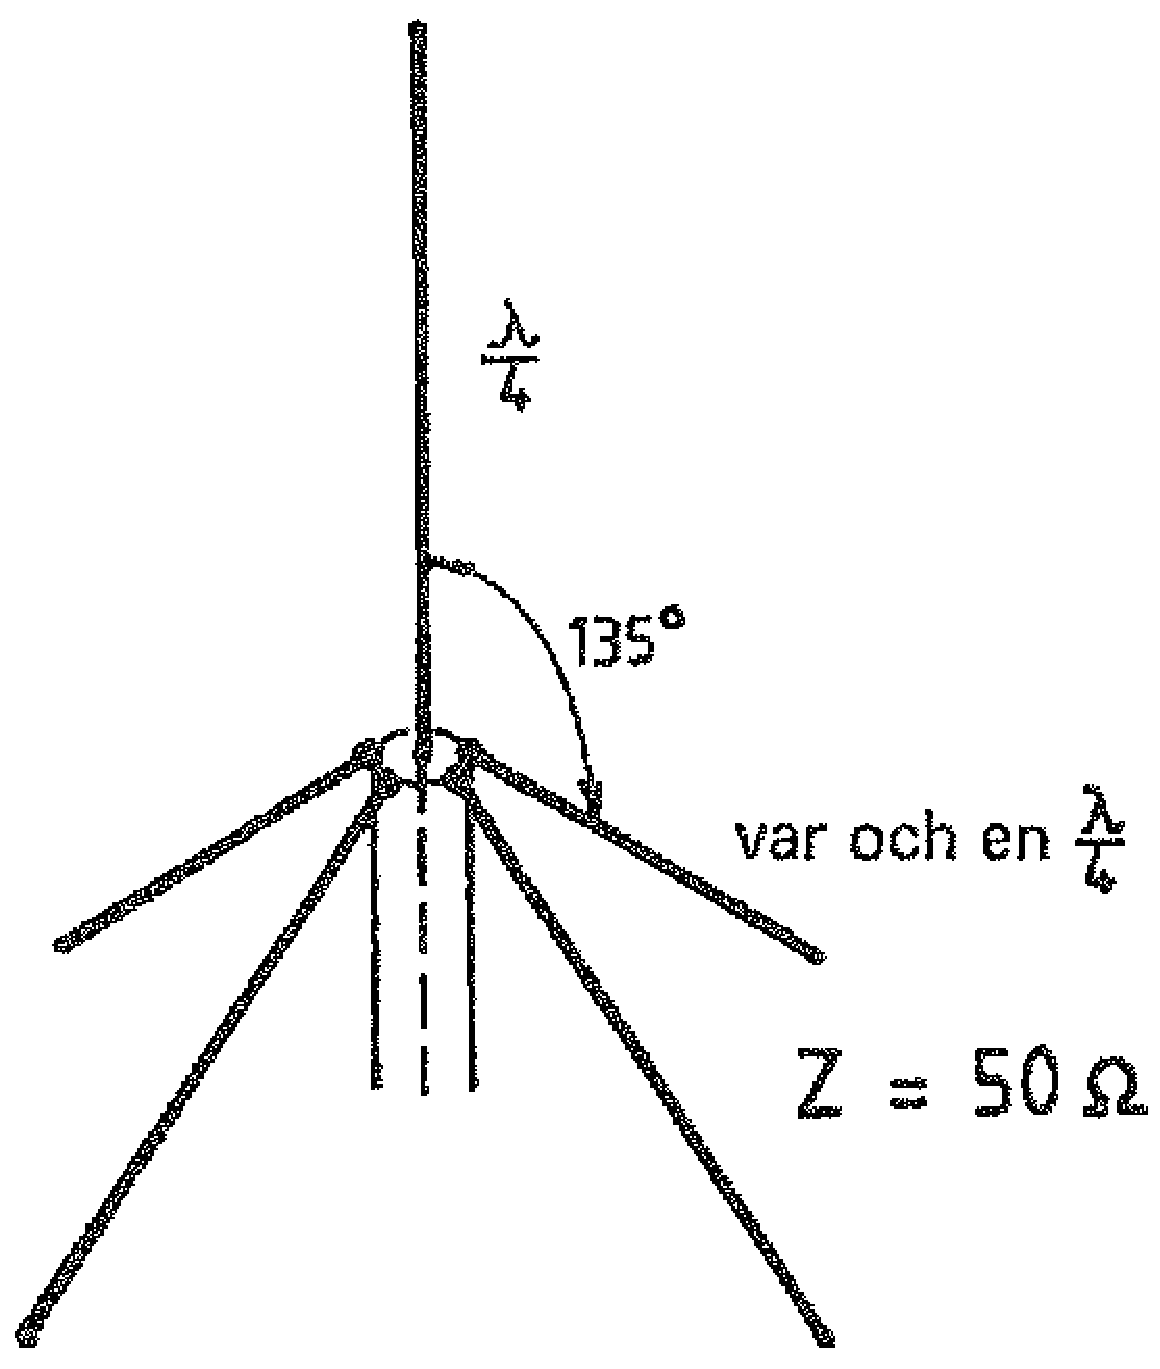
\includegraphics[width=0.5\textwidth]{images/cropped_pdfs/bild_2_6-13.pdf}
  \caption{GP-antenn}
  \label{fig:bildII6-13}
\end{wrapfigure}

Bild \ref{fig:bildII6-13} visar en \emph{jordplanantennen} eller
\emph{GP-antennen} (eng. \emph{Ground plane antenna}) består av en
lodrät strålare som den ena polen och flera sammankopplade
\(\lambda/4\)-radialer eller markplanet som den andra polen.

GP-antennen är rundstrålande och har vertikal polarisering.
Dess relativt flacka utstrålning, i jämförelse med en horisontell antenn,
gör den lämpad för långa distanser.
Av mekaniska skäl används den mest på högre frekvenser (14~MHz och högre).

Med horisontella radialer som jordplan är matningsimpedansen ca 35~\(\Omega\).
För att få god impedansanpassning, till exempel till en 50~\(\Omega\) koaxialkabel
som matarledning, görs radialerna sluttande nedåt i en lämplig vinkel.

Koaxialkabelns innerledare ansluts till antennen och kabelskärmen till
radialerna.

Om antennen placeras omedelbart ovan markytan, kan marken användas som
jordplan, särskilt om dess elektriska ledningsförmåga är god.

Om antennelementet inte har en elektrisk längd av \(\lambda/4\), kan
längden anpassas elektriskt på liknande sätt som beskrivits tidigare i
kapitel \ref{elektrisk förlängning} för dipolantenner.
Bild \ref{fig:bildII6-14} illustrerar detta.

\begin{figure}
  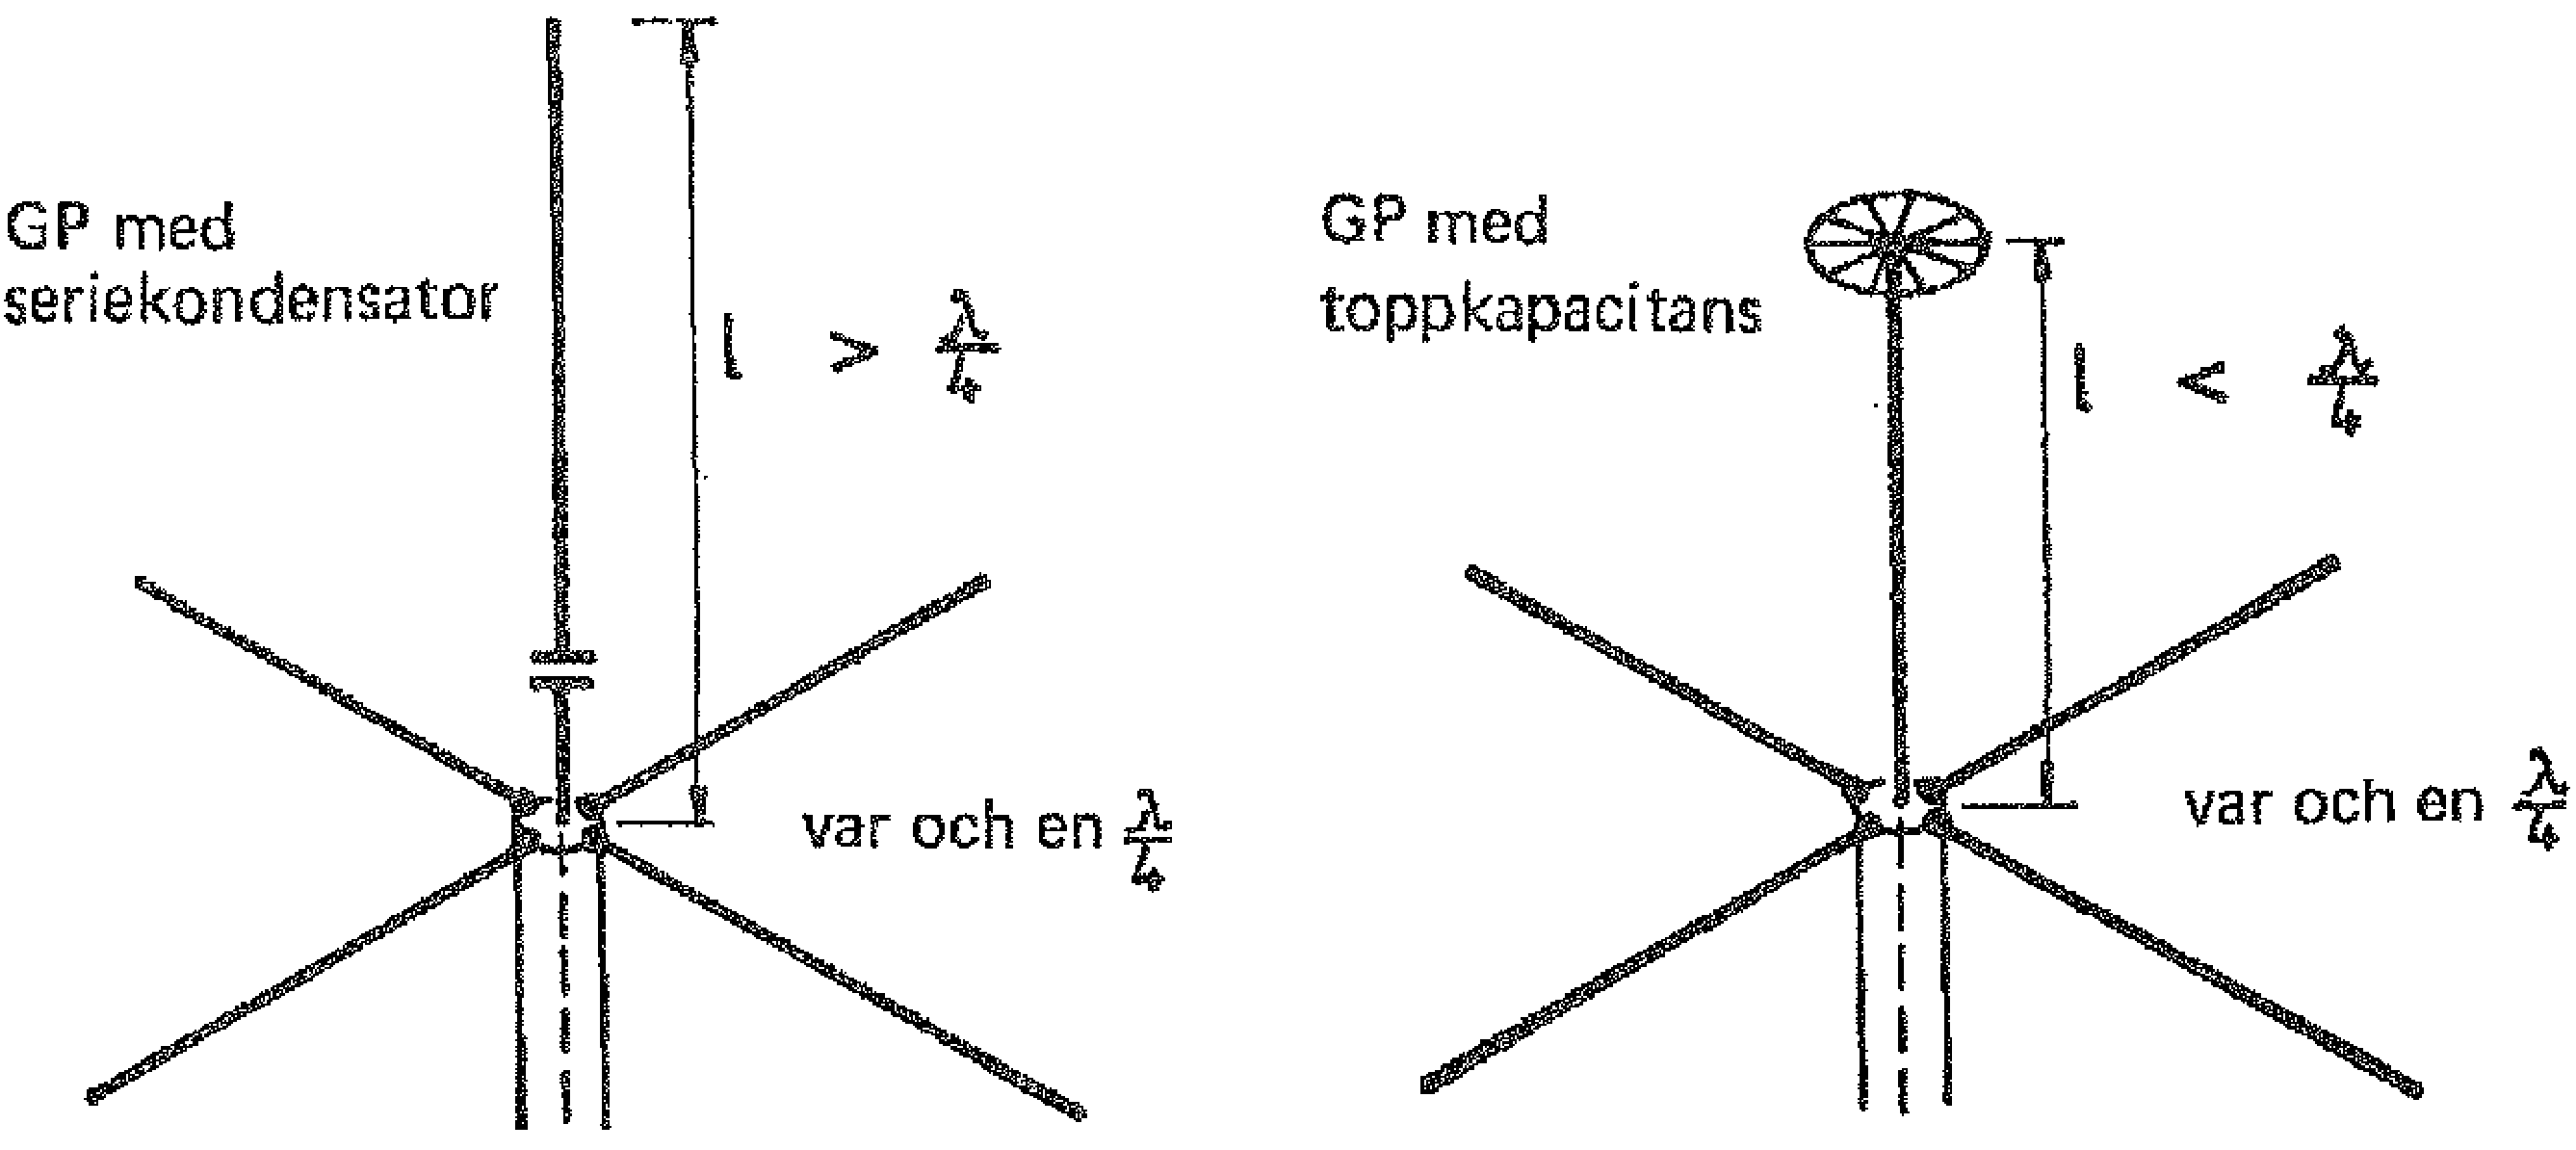
\includegraphics[width=\textwidth]{images/cropped_pdfs/bild_2_6-14.pdf}
  \caption{GP-antenner med elektrisk längdanpassning}
  \label{fig:bildII6-14}
\end{figure}

\subsection{Flerbands GP-antenner}
\index{GP-antenn}
\index{antenn!GP}

En GP-antenn kan fås att fungera på flera band genom inbyggnad av en spärrkrets
i antennelementet för tillkommande band och av jordplansradialer med anpassad
längd eller med spärrkretsar även i jordplanet för de banden.
Detta illustreras i bild \ref{fig:bildII6-15} för fem olika band.

Antennen fungerar som \(\lambda/4\) GP-antenn åtminstone på de lägsta banden.
Den mekaniska längden på en flerbands GP för kortvåg blir kort, 4 à 6,5~meter,
vilket på de lägre banden innebär dålig verkningsgrad och liten bandbredd.
Jämför med SVF-kurvorna på bild \ref{fig:bildII6-15}.
Flerbands GP-antenner för upp till sju kortvågsband tillverkas.

\begin{figure}
  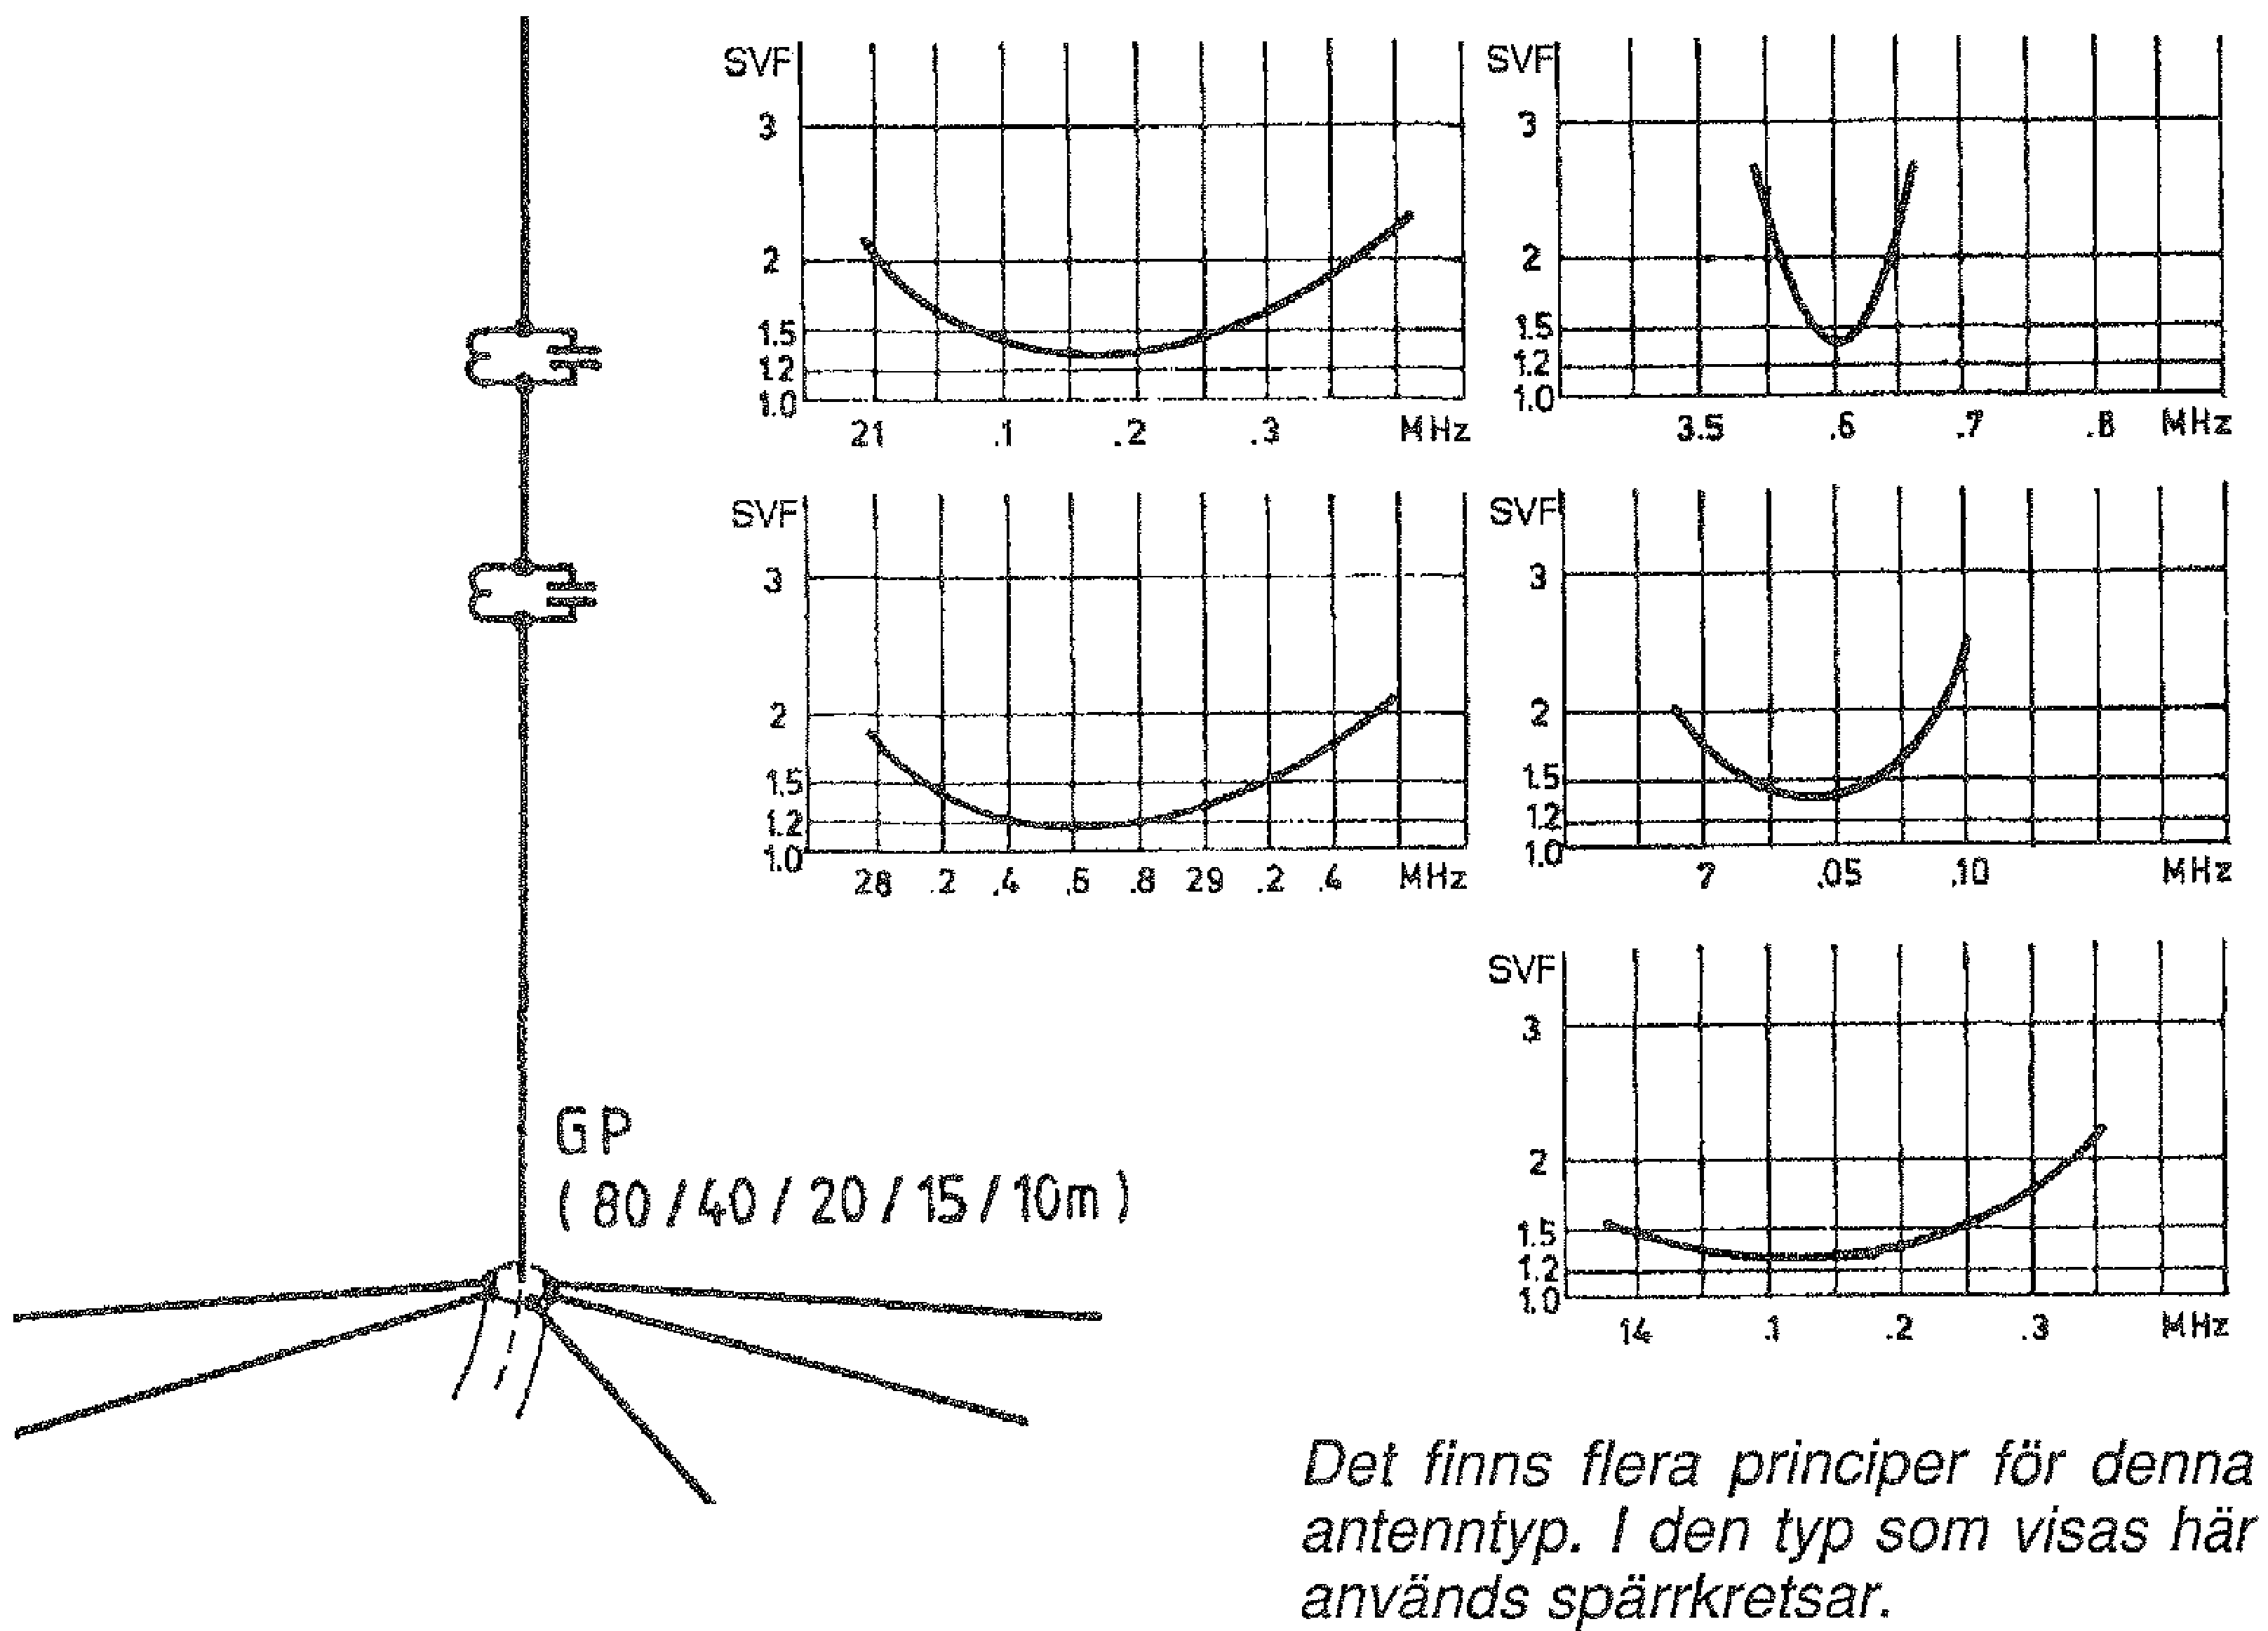
\includegraphics[width=\textwidth]{images/cropped_pdfs/bild_2_6-15.pdf}
  \caption{SVF-kurvor för flerbands GP-antenn}
  \label{fig:bildII6-15}
\end{figure}

\subsection{Flerbands halvvågsantenner}
\textbf{
HAREC a.\ref{HAREC.a.6.1.7}\label{myHAREC.a.6.1.7}
}
\label{W3DZZ}

En vanligt förekommande flerbandsantenn är W3DZZ-antennen (namnet
efter konstruktörens anropssignal) som visas i bild \ref{fig:bildII6-16}.
Det är en horisontellt upphängd dipolantenn för 80, 40, 20, 15 och
10~m-banden.

W3DZZ-antennen är ca 33,6~meter lång och har två spärrkretsar,
symmetriskt utplacerade omkring matningspunkten.
Matningen sker med koaxialkabel och balun.

Antennen har en matningsimpedans av ca 60~\(\Omega\) på 80- och
40-metersbanden På de högre banden är anpassningen inte optimal --
matningsimpedansen stiger där upp till ca 100~\(\Omega\).
Många använder bl.a. av den anledningen inte W3DZZ-antennen på höga
kortvågsband utan föredrar där en flerbandig GP-antenn eller en riktantenn
(yagi, quad m.fl.).

\begin{figure}
  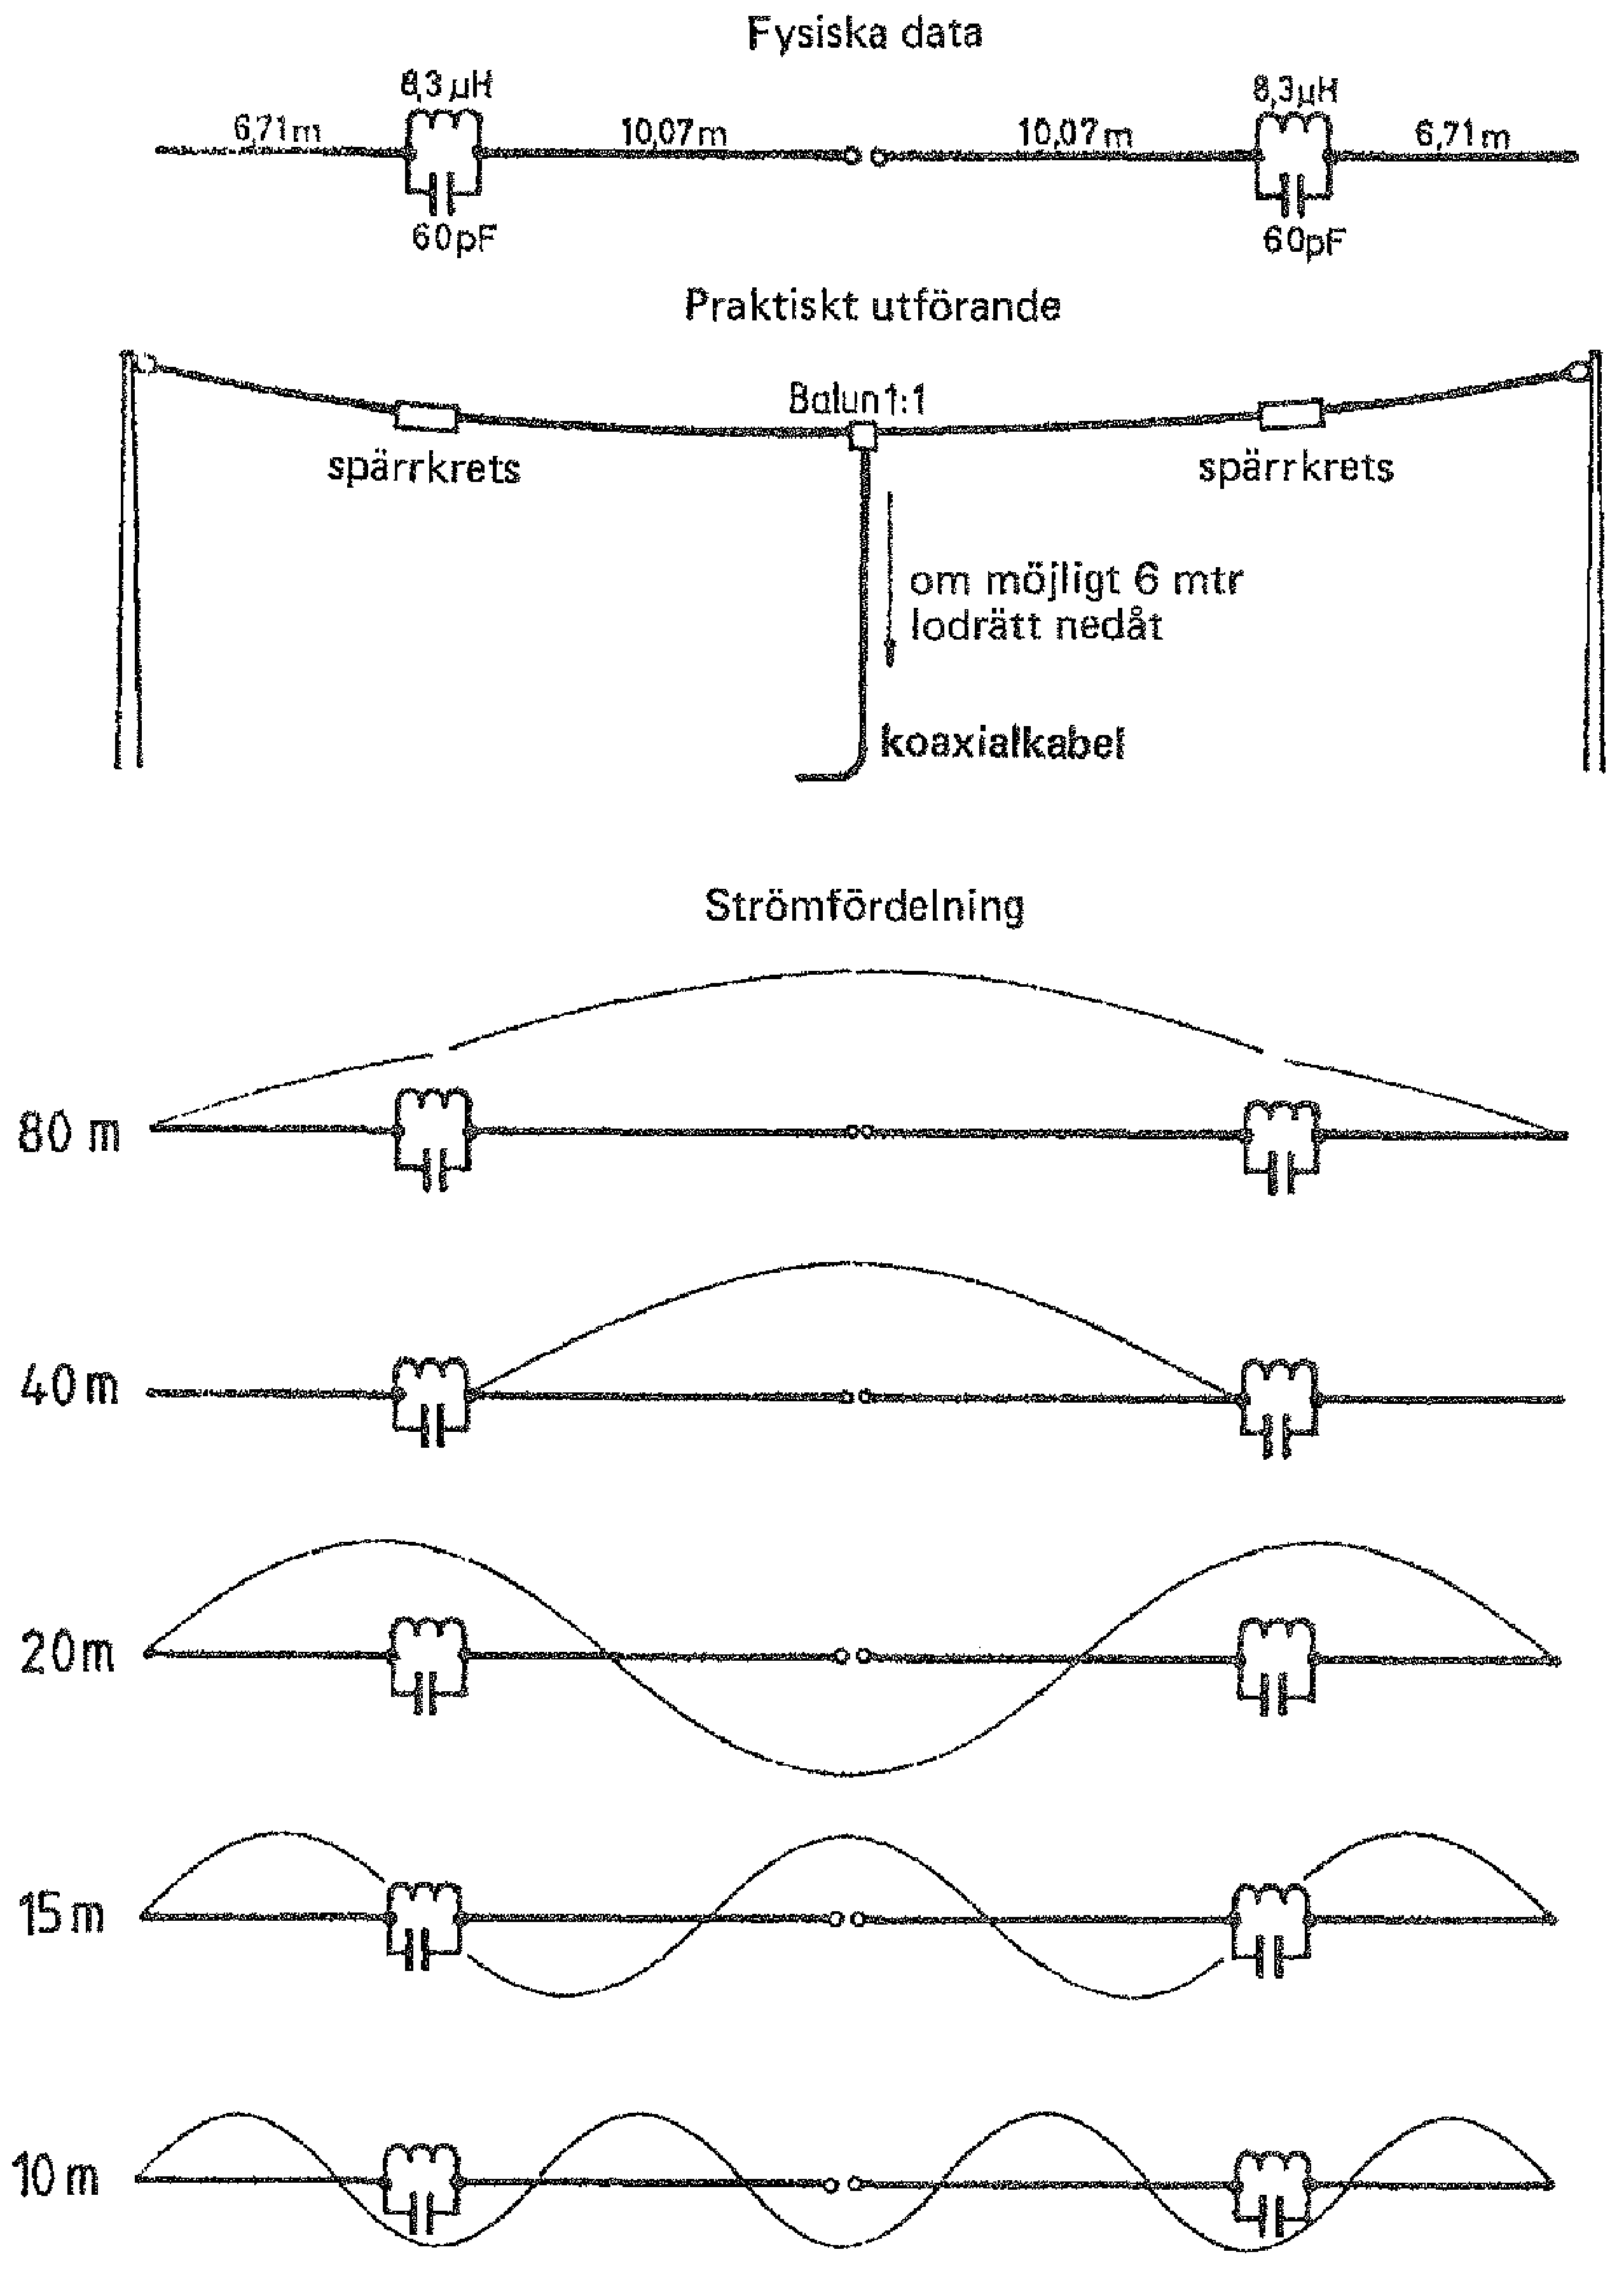
\includegraphics[width=\textwidth]{images/cropped_pdfs/bild_2_6-16.pdf}
  \caption{W3DZZ-antennen}
  \label{fig:bildII6-16}
\end{figure}

W3DZZ-antennens arbetssätt:
\begin{itemize}
\item 80 m-bandet \\ Hela antennen fungerar som en \(\lambda/2\)-dipol med
  resonansfrekvensen 3,7~MHz.
  Den mekaniska längden är \(2 \cdot 16,8\) meter och förlängs elektriskt med
  induktanserna i spärrkretsarna, vilka f.ö. är ur resonans på detta band.

\item 40 m-bandet \\ Spärrkretsarna är i resonans och ''kopplar bort''
  antenndelen utanför dem.
  Delen där innanför fungerar som en \(\lambda/2\)-dipol med resonansfrekvensen
  7,05~MHz.

\item 20 m-bandet \\ Hela antennen fungerar som \(3\lambda/2\)-dipol
  med resonansfrekvensen 14,1~MHz.

\item 15 m-bandet \\ Hela antennen fungerar som \(5\lambda/2\)-dipol
  med resonansfrekvensen 21,2~MHz.

\item 10 m-bandet \\ Hela antennen fungerar som \(7\lambda/2\)-dipol
  med resonansfrekvensen 28,4~MHz.
\end{itemize}
